%%%%%%%%%%%%%%%%%%%%%%%%%%%%%%%%%%%%%%%%%%%%%%%%%%%%%%%%
%
% Change the option between square brackets
% depending on the document you have to write:
%
% proposal    for the initial proposal
% review      for the literature review
% progress    for the progress report
% final       for the final report
% 
%%%%%%%%%%%%%%%%%%%%%%%%%%%%%%%%%%%%%%%%%%%%%%%%%%%%%%%%

\documentclass[final]{cmpreport}
\makeatletter
\input{t1pcr.fd}
\makeatother
\setlength{\footnotesep}{3ex}
\usepackage{listings}
\usepackage{pgfplots}
% Some package I am using. You may not need them
%
\usepackage{rotating}
\usepackage{subfloat}
\usepackage{float}
% packages for algorithms
\usepackage{amsmath}
\usepackage{algorithm}
\usepackage[noend]{algpseudocode}




%\setkeys{Gin}{draft}

%%%%%%%%%%%%%%%%%%%%%%%%%%%%%%%%%%%%%%%%%%%%%%%%%%%%%%%%
%
%  Fill in the fields with:
%
%  your project title
%  your name
%  your registration number
%  your supervisor's name
%
%%%%%%%%%%%%%%%%%%%%%%%%%%%%%%%%%%%%%%%%%%%%%%%%%%%%%%%%
\title{AI search algorithms for the solution of puzzles}

%%%%%%%%%%%%%%%%%%%%%%%%%%%%%%%%%%%%%%%%%%%%%%%%%%%%%%%%
%
% The author's name is ignored if the following command 
% is not present in the document
%
% Before submitting a PDF of your final report to the 
% project database you may comment out the command
% if you are worried about lack of anonimity.
%
%%%%%%%%%%%%%%%%%%%%%%%%%%%%%%%%%%%%%%%%%%%%%%%%%%%%%%%%
\author{Luke Garrigan}


\registration{100086495}
\supervisor{Dr Pierre Chardaire}
%%%%%%%%%%%%%%%%%%%%%%%%%%%%%%%%%%%%%%%%%%%%%%%%%%%%%%%%
%
% Fill in the field with your module code.
% this should be:
%
% for BIS            -> CMP-6012Y
% for BUSINESS STATS -> CMP-6028Y
% for other students -> CMP-6013Y
%
%%%%%%%%%%%%%%%%%%%%%%%%%%%%%%%%%%%%%%%%%%%%%%%%%%%%%%%%
\ccode{CMP-6012Y}


\summary{



}

\acknowledgements{
	
FIrstly, I would like to express my sincere gratitude to my advisor Dr. Pierre Chardaire for the patience, guidance, wisdom and brilliance he has provided throughout my final year. I have been extremely lucky to have
a supervisor who cared so much about my work, and who responded to my questions and queries so
promptly.

}

%%%%%%%%%%%%%%%%%%%%%%%%%%%%%%%%%%%%%%%%%%%%%%%%%%%%%%%%%%%%%%%%%%
%
% If you do not want a list of figures and a list of tables
% to appear after the table of content then uncomment this line 
%
% Note that the class file contains code to avoid
% producing an empty list section (e.g list of figures) if the 
% list is empty (i.e. no figure in document).
%
% The command also prevents inserting a list of figures or tables 
% anywhere else in the document
%
% Some supervisors think that a report should not contain these
% lists. Please ask your supervisor's opinion.
%
%%%%%%%%%%%%%%%%%%%%%%%%%%%%%%%%%%%%%%%%%%%%%%%%%%%%%%%%%%%%%%%%%%
%\nolist,

%%%%%%%%%%%%%%%%%%%%%%%%%%%%%%%%%%%%%%%%%%%%%%%%%%%%%%%%%%%%%%%%%%
%
% Comment out if you want your list of figures and list of
% tables on two or more pages, in particular if the lists do not fit 
% on a single page.
%
%%%%%%%%%%%%%%%%%%%%%%%%%%%%%%%%%%%%%%%%%%%%%%%%%%%%%%%%%%%%%%%%%%
\onePageLists

\begin{document}



\section{Introduction}



 In computer science a search algorithm is a series of steps that can be used to find a desired state or a path to a particular state. In most scenarios there will be additional constraints that will need to be fulfilled such as the time taken to reach the desired state, memory availability, maximum number of moves. The main difference between informed search and uninformed search is the use of heuristic functions that guide the search towards the goal while avoiding non-promising paths \cite{felner2015early}. Informed search algorithms such as A* \cite{hart1968formal}, IDA* \cite{korf1985depth} are analysed in this paper with various heuristics including Manhattan distance, linear conflict \cite{hansson1985generating} and pattern databases (PDB) \cite{culberson1996searching}. A comparison between informed and uninformed search is made along with an in-depth analysis of different heuristics for specific problem domains such as the sliding-tile puzzle, Towers of Hanoi and the Rubik's cube.

 A classic example in the AI literature of pathfinding problems are the sliding-tiles puzzles such as the $3\times3$ 8-puzzle, the $4\times4$ 15-puzzle and the $5\times5$ 24-puzzle. The 8-puzzle consists of a $3\times3$ grid with eight numbered square tiles and one blank. The blank is used to slide other tiles in which are horizontally or vertically adjacent into that position in an attempt to reach the goal state. The objective is to rearrange the tiles from some random configuration to a specified goal configuration. The number of possible solvable states for the 8-puzzle is $9!/2=181440$ so can be solved by means of brute-force search. However for the 15-puzzle with $16!/2\approx1.05\times10^{13}$ and 25-puzzle with $25!/2\approx7.76\times10^{24}$ a more sophisticated informed search is required.
 
 The Towers of Hanoi puzzle consists of $3$ pegs and $n$ discs all of varying sizes. The discs are initially stacked on the leftmost peg in decreasing order of size with the largest on the bottom. The task is to move all discs from the initial peg to the goal peg without violating two constraints: Only the top disc of any peg can be moved and a larger disc can never be placed on top of a smaller disc. For the $3$ peg problem a simple recursive algorithm can be used to find the solution in the minimum number of moves, however, for the $4$ peg problem (TOH4) the recursive algorithm doesn't find the goal state optimally. The recursive algorithm works by initially moving the $n-1$ smallest discs to the intermediate peg, then moving the $n-1$ largest disc to the goal peg, then move the $n-1$ smallest discs from the intermediate peg to the goal peg. Finding shortest path with this algorithm is not possible with TOH4 because there are two intermediate pegs rather than one and without priori there is no way to determine which peg should be used over the other. This implies the use of systematic search to find the optimal path.
 
 
 

 


\section{Relevant Literature And Context}
The following review discusses a complete definition and overview of the search algorithms implemented in the project, discussing their strengths and weaknesses and their applicability to the sliding-tile puzzle. 
\subsection{Uninformed Search}
Uninformed or brute-force search is a general problem-solving technique that consists of systematically enumerating all the possible states for a given solution and checking to see whether that given state satisfies the problem's statement. All that is required to execute a brute-force is some legal operators, an initial state and an acknowledged goal state. Uninformed search generates the search tree without using any domain specific knowledge
\subsubsection{Completeness and Optimality}
 Often in search the input may be an implicit representation of an infinite graph. Given these conditions, a search algorithm is characterised as being complete if it is guaranteed to find a goal state provided one exists. Breadth-first search is complete and when applied to infinite graphs it will eventually find the solution. Depth-first search is not complete and may get lost in parts of the graph that do not contain a goal state.
\subsubsection{Breadth-First Search}
Breadth-first search is one of the simplest algorithms for searching a graph, it expands the nodes in a tree in the order of their given distance from the root, so it expands all the neighbouring nodes before going to the next level of the tree. The algorithm doesn't trawl to the deeper levels of the tree without first expanding the lower levels thus ensures the finding of the shortest path. The amount of time used by breadth-first search is linear to the number of nodes expanded, since each node can be generated in constant time, and is a function of the branching factor $b$ and the solution depth $d$. Since the number of nodes at level $d$ is $b^d$, the total number of nodes generated in the worst case is $O(b^d)$. \citep{DBLP:journals/mima/Korf95}. The space requirement of breadth-first search is its largest deficiency. The 8-tile has a search space of $9!/2=181,400$ states with a maximum number of 31 moves to solve. In terms of practicality, with larger problem states such as the 15-tile puzzle a breadth-first search will exhaust the available memory rather quickly with its $16!/2 = 10,461,394,944,000$ states and a maximum number of 80 moves to solve.



The operations of enqueuing and dequeuing take O.1/ time, and so the total time devoted to queue
operations is O.V /. Because the procedure scans the adjacency list of each vertex
only when the vertex is dequeued, it scans each adjacency list at most once. Since
the sum of the lengths of all the adjacency lists is ‚.E/, the total time spent in
scanning adjacency lists is O.E/. The overhead for initialization is O.V /, and
thus the total running time of the BFS procedure is O.V C E/. Thus, breadth-first
search runs in time linear in the size of the adjacency-list representation of G.


\subsubsection{Depth-First Search}
Depth-first search (DFS) addresses the limitations of breadth-first by always generating next a child of the deepest unexpanded node. Breadth-first search manages the list as a first-in first-out queue, whereas depth-first search treats the list as a last-in first-out stack. Depth-first search is implemented recursively, with the recursion stack taking the place of an explicit node stack. Given a starting state, depth-first search stores all the unvisited children of that state in a stack. It then removes the top state from the stack and adds all of the removed states children to the stack. Depth first search generates a long sequence of moves, only ever reconsidering a move when it reaches the end of a stack, this can become a serious problem given a graph of significant size and there's only one solution, as it may end up exploring the entire graph on a single DFS path only to find the solution after looking at each node. Worse, if the graph is infinite the search might not terminate.



\subsubsection{Depth-Limited Search}
Depth-Limited search is DFS with a cut-off depth, this prevents the search from running forever provided the limit isn't set to infinite. The algorithm is not complete as the solution depth could be greater than the cut-off depth and it is not optimal. The algorithm is second procedure shown in Algorithm~\ref{DFID}.


  
\subsubsection{Depth-First Search Iterative Deepening}
Depth-First Iterative-Deepening (DFID) is an extension of depth-first search, it combines breadth-first search's completeness and depth-first search's space efficiency. DFID has a maximum depth by using DLS; searching all possibilities up to the specific depth and if it doesn't find the goal state it increases the depth increases. DFID performs depth-first search to depth one, then starts over and executes a depth-first search to depth two and continues deeper and deeper until a solution is found. The complexity of DFID is only O(d) where d is the depth, this is because at a given point it is executing only a depth-first search and saving only a stack of nodes. DFID ensures that the shortest path to the goal state will be found as does breadth-first search \citep{DBLP:conf/otm/MeissnerB11}.








\subsection{Informed Search}
Uninformed search often expands states that pursue a direction alternative to the goal path, which can lead to searches taking an extensive amount of time and/or space. Informed search attempts to minimise this by producing intelligent choices for each selected state. This implies the use of a heuristic function which evaluates the likelihood that a given nodes is on the solution path. A heuristic is a function that ranks possible moves at each branching step to decide which branch to follow. The goal of a heuristic is to produce a fast estimation of the cost from the current state to the desired state, the closer the estimation is to the actual cost the more accurate the heuristic function. In the context of the sliding-tile puzzle, to find best move from a set configuration the heuristic function is executed on each of the child states, the child state with the smallest heuristic value is chosen.
 


\subsubsection{Admissible Heuristics}
A heuristic function is said to be admissible if it never overestimates the cost of reaching the goal, i.e the estimated cost to the goal from the current node is not higher than the lowest possible cost from the current node. The lowest possible cost $h^*(n)$ is the cost of the optimal path from $n$ to a goal node $G$. The heuristic function $h(n)$ is admissible if $0 \leq h(n) \leq h^*(n)$; admissible heuristic functions are optimistic meaning they are lower bounds on the actual cost.

\subsubsection{Consistent Heuristics}
 A heuristic function is said to be consistent if the cost from the current node $n$ to a successor node $p$, plus the estimated cost from the successor node to the goal state is less than or equal to the estimated cost from the current node to the goal node $h(n)\leq c(n,p) + h(p)$, where $c(n,p)$ is the cost of reaching node $p$ from $n$ and the heuristic value of the goal $G$ is zero $h(G)=0$ (Figure 2). 


\begin{figure}[ht]
	\centering
	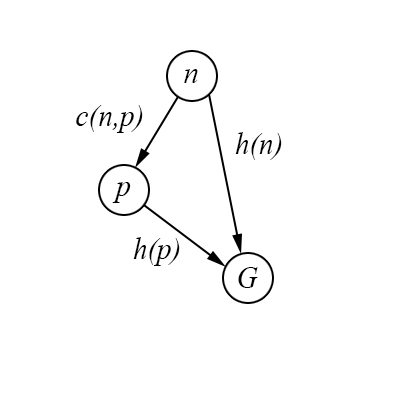
\includegraphics[width=0.4\textwidth]{consistent}
	\captionsetup{justification=centering}
	\caption{Consistent Heuristics Diagram}
\end{figure}



\subsubsection{Manhattan Distance}
Manhattan distance is the classic heuristic function for the sliding-tile puzzles, for each tile in the puzzle the Manhattan distance counts the number of grid units between its current location
and its goal location and summing these values for all tiles. Manhattan distance is a lower bound on actual solution length, because every tile must move at least its Manhattan distance, and each move only moves one tile. The Manhattan distance is a lower bound for the number of moves required to solve an occurrence of the sliding-tile puzzle, since every tile must move at least as many times as its distance to its goal position. \citep{DBLP:conf/ccgrid/LinnertSB14}. 

$$h(n)= \sum_{all\ tiles}^{}distance(tile, goal\ position)$$



	


\subsubsection{Linear-Conflict Heuristic}
Linear-conflict heuristic is an improvement to the Manhattan distance, it applies when two tiles are positioned in their desired row or column but are reversed relative to
their goal positions, meaning a given tile must move out of the row or column in order to let the other pass. If there is a linear conflict then an extra two moves will be added to the total sum as the tile which must move, has to transition out of the row or column and then back into its desired position. These two extra moves are not included in the Manhattan distance so can be added to the total without violating admissibility see Algorithm \ref{Linear Conflict} 


\begin{algorithm}
	\caption{Linear Conflict}\label{Linear Conflict}\cite{hansson1992criticizing}.
	\begin{algorithmic}[1]
		\State C(tj, ri) is the number of tiles in row ri with which tj is in conflict
		\State lc(s, rj) is the number of tiles that must be removed from row rj to resolve linear conflicts
		\Procedure{Linear Conflict}{$state$}	\Comment{The current puzzle configuration }
		\For{each row ri in the state s}
			\State $lc(s, ri)\gets 0$
			\For{each tile in row}
				\State determine $C(tj, ri)$
				\While{there is a non-zero C(tj, ri) value}
					\State find tk such that there is no
					\State \ \ \ \  C(tj, ri) > C(tk, ri)
					\State C(tk, ri) = 0 
					\For{every tile tj which had been in conflict with tk}
						\State C(tj, ri) = C(tj, ri) - 1 
					\EndFor
					\State lc(s, ri) = lc(s, ri) +1	
				\EndWhile
			\EndFor
		\EndFor
		\State \textbf{return} $total$\Comment{The heuristic is the total}
		\EndProcedure
	\end{algorithmic}
\end{algorithm}


\begin{figure}[ht]
	\centering
	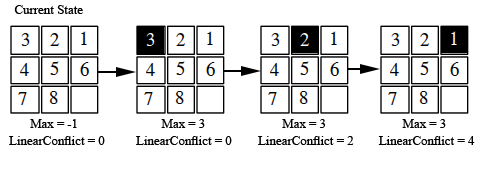
\includegraphics[width=0.9\textwidth]{linear}
	\captionsetup{justification=centering}
	\caption{Calculating Linear Conflict}
\end{figure}



\subsubsection{A* Algorithm}
A* search is a combination of lowest-cost-first and best-first searches that considers both path cost and heuristic information in its selection of which path to expand. For each path on the frontier, A* uses a heuristic function. This allows A* search to ensure the prioritisation of states in which are more likely to result in a low-cost goal state. The calculation of the heuristic value is dependent on the problem that is being solved. For example, for problems which aim to reach a location the Euclidean distance between the state and the goal is often used as the heuristic. 

The A* algorithm uses $cost(p)$, the cost of the path found, as well as the heuristic function $h(p)$, the estimated path cost from the end of $p$ to the goal. As A* uses admissible heuristic it will always find solutions in the order of their cost. \citep{DBLP:journals/ker/Brewka96}.  A* uses breadth-first traversal thus uses large chunks of memory in comparison to applications that use depth-first traversal. The performance of A* is also heavily reliant on the accuracy of the heuristic.






\subsubsection{Iterative Deepening A*}
Iterative-deepening A* (IDA*) eradicates the memory complication of A* by using depth-first traversal, without sacrificing solution optimality at the cost of increasing the time taken. Each iteration of A* is a complete depth-first search that keeps track of the cost, $f(n) = g(n) = h(n)$, of each node generated. If an expanded node's cost generated exceeds a threshold for that iteration, its path is cut off and the search backtracks before continuing. IDA* ranks states the same way as A*: The expected cost of a state is the cost of reaching said state plus the heuristic's estimate of the cost of reaching the nearest goal state. The maximum expected cost is assigned to the heuristic cost of the starting state, states which have a lower cost than the starting state are traversed and states with a higher expected cost are discarded. 


If IDA* has searched all states lower than the current maximum without finding the goal state then it increases the maximum to the lowest value of the discarded states and begins the search again. The goal state is admissible, the current maximum cost will never be higher than the lowest cost solution, thus IDA* with an admissible heuristic will always find the lowest cost solution.  IDA* searches many nodes multiple times thus is slower than A*. Hence, A* should be used on smaller applications with lower memory requirements.


The time complexity of IDA* is measured by the number of nodes expanded, provided each node can be expanded and its successors evaluated in constant time, the asymptotic time complexity of IDA* is the total nodes expanded. Otherwise it is the product of the total number of nodes and the time taken to expand each. Provided the heuristic is consistent (see 4.2), IDA* must expand all nodes with the $f$ value less than or equal to $c$ which  is the cost of an optimal solution $f(n) \leq c$. On the final iteration of IDA* the cost threshold is equal to $c$, the cost of an optimal solution.\citep{DBLP:journals/ai/KorfRE01}.
\subsection{Pattern Databases}
A Pattern Database (PDB) stores a collection of solutions to sub-problems that must be achieved to solve the overall problem. They then used as admissible heuristics implemented as lookup tables that store the lengths of optimal solutions for sub-problem instances. \citep{DBLP:journals/jair/FelnerKMH07}.

\subsubsection{Non-Additive Pattern Databases}\label{Section:nonadditive}
For any configuration of the sliding tile puzzle, the minimum number of moves required to solve a subset of the tiles is evidently a lower bound on the number of moves needed to solve the puzzle \cite{felner2004additive}.





The initial PDB applied to the fifteen tile as shown in Figure \ref{fig:fringe} is the fringe pattern. The heuristic is estimated dependent on the current positions of the fringe tiles and the blank, however is independent of the positions of the other tiles. These values are precomputed and stored in a lookup table and are called upon when a heuristic estimate is needed. The total number of possible permutations of fringe tiles and blank is $16!/(16-8)!=518,918,400$. 

To retrieve all possible permutations of the Fringe tiles a single breadth-first search must be executed, commencing at the goal state. Tiles which are not fringe are all equivalent, in the database the positioning of the fringe tiles and the blank are stored along with the number of moves taken to get to that state. Using IDA* an optimal solution can be found for the 15-puzzle as the heuristic estimate is optimistic, meaning admissible. To retrieve the value from the lookup table an index must be made from the positioning of the Fringe tiles and the blank, this value is then used as the heuristic estimate for the given state.

\cite{culberson1998pattern} show that it is possible to use the Fringe PDB and the Corner PDB to determine the heuristic estimate by taking the maximum of the two values, Figure \ref{fig:fringe} displays both the Fringe and the Corner pattern. They explain how there are other viable patterns but intuitively the Fringe and Corner pattern are likely the best at providing the lower bounds for the search. Their reasoning for this assumption was by analysing the work left once the subset had been solved, after solving the fringe tiles only an 8-puzzle remains. Their experiments showed that the best results were from pattern databases that reduced the problem to a simpler one whose solution requires little or no interference with the placing of the pattern, both Fringe and Corner satisfy this.



\begin{figure}[ht]
	\centering
	\captionsetup{justification=centering}
	
	\begin{subfigure}{.3\textwidth}
		\centering
		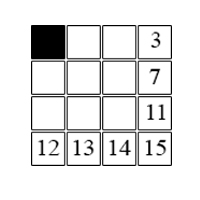
\includegraphics[width=.9\textwidth]{fringe}
	\end{subfigure}%
	\begin{subfigure}{.3\textwidth}
		\centering
		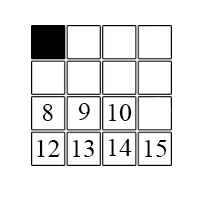
\includegraphics[width=.9\textwidth]{corner}
	\end{subfigure}
	\caption{Fringe and Corner patterns for 15 }
	\label{fig:fringe}
\end{figure}



The major issue is space required to store all possible states. When considering the 15 tile: provided each row in the database is 1 byte and there are 519,914,400 rows that's a total of 519Mb, and the time taken to perform the breadth-first search is extensive. Scalability is another issue regarding non-additive pattern databases, if scaled to the twenty-five tile puzzle and performed the same calculations for taking the fringe: $25!/(25-10)!=1.1861676e+13$, provided each row in the database is 1 byte as previously stated, the total is roughly 12 Terabytes worth of storage.







\subsubsection{Statically-Partitioned Additive Database Heuristics}
Rather than taking the maximum of the two pattern databases a better option would be to sum the values without violating admissibility and tightening the lower bound. There are two methods to do this: statically-partitioned additive pattern databases and dynamically-partitioned additive pattern databases. In order to create a statically-partitioned additive database for the sliding tile puzzle, the tiles were partitioned into disjoint groups, meaning each tile is placed in a specified group and only appears in that group. The same method as explained in \ref{Section:nonadditive} for finding all the states was computed for each subset; a breadth-first search from the goal state with all possible configurations of each tile in the disjoint groups and the number of moves required to get to the goal state. For a particular state in the search, for each position of the tiles an index was computed for the corresponding row in the database, then retrieved the number of moves required to solve the tiles in that group and added this value to each value of the other disjoint groups. The summed total of these values will always be equal to or larger than the Manhattan distance of the state as it considers the interactions between tiles within a given subset.	

Non-additive pattern databases include all the moves required to solve a pattern, including non-labelled tiles. Therefore, two PDB values cannot be added together as an admissible heuristic as moves counted in one PDB could move tiles in the other, meaning the same move would be counted twice. Whereas only the moves in a particular group are counted in additive databases, so the sum can be taken off the pattern values.


\begin{figure}[ht]
	\centering
	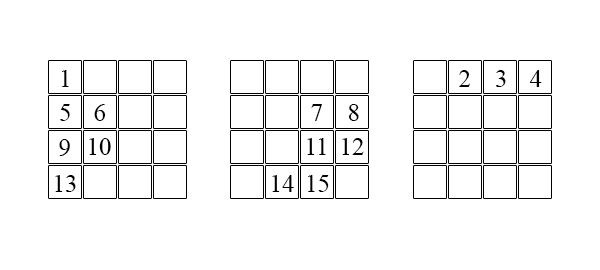
\includegraphics[width=0.9\textwidth]{15tile}
	\captionsetup{justification=centering}
	\caption{6-6-3 Partioning}
	\label{fig:partitioning}
\end{figure}


\subsection{Summary}

\subsubsection{Evaluation Of Uninformed Searches}
Althought DFS memory requirement is linear and it has less time and space complexity to BFS, often DFS induces the possibility of traversing down the left-most path forever, it is also not guaranteed to find the solution.

Depth-first iterative deepening is beneficial as it avoids infinite cycling, it obtains the same result as BFS whilst saving memory, however it is very slow as it has to repeatedly expand nodes it has already visited. DFID is only really beneficial when the solution depth is known, else it would have to trawl through all possibilities up to the solution depth and then through all possibilities at the solution depth until it reaches the goal. It is unlikely for the sliding-tile puzzle that the user knows the solution depth, thus implies ample execution time to find the goal state. Theoretically DFID could be used on much more difficult problems which have a larger search space, such as the 15 or 25 tile, but the time taken to find the solution outweighs any benefits. 

Breadth-first search is very fast when considering the 8-tile puzzle as the search space is small, however it uses too much memory to be useful with larger problems such as the 15-tile puzzle. If there are multiple solutions, it will find the solution with the least steps.

\subsubsection{Evaluation of Informed Searches}
Provided the heuristic function is admissible both informed search algorithms will find the optimal path to the goal state. The main drawback of the A* algorithm is its memory requirements; it must store all the visited states in the open set. Although the algorithm runs successfully on small problems such as the eight puzzle, it exhausts available memory rather quickly for the fifteen puzzle, Section \ref{Experimental Results} displays the testing results of this memory usage for random states. 

IDA* on the other hand eliminates the memory constraints of A*, by performing a series of depth-first searches and not needing to store the open set. IDA* was chosen for solving larger search spaces, tested using a number of different heuristics. 




\section{Design}
This section describes the design of the program and specifically the various search algorithms and the appropriate steps required based on the literature review. Pseudo code for each algorithm has also been constructed to form a structure for the implementation.
\subsection{Class Diagram}
Figure \ref{figure:classDiagram} shows a shortened version of the implementation, other algorithms also included in the program are DFS and DFID. Other classes used to construct testing states were not included in the diagram for simplicity, these classes include \textit{RandomStates} which given a particular puzzle returns random solvable states and \textit{Testing} which is used primarily for testing algorithms and determining the number of nodes they expand, the time taken to solve the problem, number of moves and many other statistical values, used extensively in Section \ref{Experimental Results}


\subsection{Representing the state}
The first step to solving the sliding tile puzzle is determining the best way to store a particular state. There were three elements that needed to be considered: the order of the tiles, the dimensions of the puzzle and the position of the blank. Puzzle configurations were stored using an array, the blank tile was represented by a 0 and the dimensions of the puzzle can be found from the length of the array (square root of the length, provided the state has an equal height and width). The positioning of the blank is important as it is needed for finding legal moves; every tile must push into the blank and computing the position of the blank each iteration would be costly.

Additional fields including the parent state were stored for the ability to traverse the path the algorithm took back to the initial state, the direction that each state took is also stored. Each state contains a heuristic array which is the same length as the puzzle state, each position in the heuristic array represents the number of estimated moves for that given tile to reach its goal state. It would be costly to continually compute the heuristic estimate of every tile in the current configuration: the heuristic array is filled by an initial heuristic calculation and then each state after only computes the heuristic for the previously moved tiles. Figure \ref{figure:classDiagram} shows the class diagram of project.

The State class also contains the number of moves from the starting state $g$, the heuristic value $h$ and $f$ or ($h+g$).

\subsection{Finding legal moves}
In order to find legal moves for the sliding puzzle, two variables must be known: the position of the blank and the dimensions of the puzzle. As shown above by representing the state, the zero value for a given state is stored and the dimensions can be easily computed. For a given state in the sliding-tile puzzle, there are 2-4 legal moves: when the blank is in a corner there are two legal moves, if the blank is against an edge but not in the corner there are three legal moves, and if the blank is surrounded by tiles in all directions there are four legal moves. The blank can move left, right, up or down, there are a elements to consider here: the blank cannot go up if its in the top row, cannot go left if its in the left-most column, right if its in the right-most column and down if its in the bottom row. In order to construct this algorithm it helped to visualise the puzzles based by their index rather than their labelled value. Figure \ref{figure:index} displays the 8 and 15-puzzle with their index representation. 
\begin{figure}[h!]
	\centering
	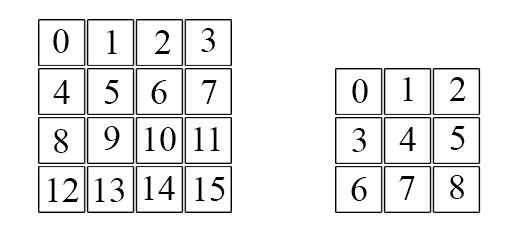
\includegraphics[width=.5\textwidth]{tile_indexes}
	\captionsetup{justification=centering}
	\caption{Sliding Tile Index Representation}
	\label{figure:index}
\end{figure}
Algorithm \ref{neighbouring_nodes} shows a procedure finding the neighbouring nodes of a particular state. Firstly, an empty list is initialised as we know there are a minimum of two possible moves from every state in the puzzle. Each possible move is tested, checking whether the empty tiles positioning satisfies the constraints, if so then a new state is built with the updated values and added to the list. Once all possible moves have been tried the list of neighbouring nodes is returned to the search algorithm.


	
\begin{algorithm}
	\caption{Finding Neighbouring States}\label{neighbouring_nodes}
	\begin{algorithmic}[1]
		\Procedure{findNeighbours}{$state$}	\Comment{The current puzzle configuration }
		\State$neighbours\gets empty list$
		\State$dimensions\gets 	dimensions\ of\ state$ \Comment{3 for 3x3, 4 for 4x4}
			\If{zeroPosition \% dimensions != 0} \Comment{left move}
			\State $left \gets updated\ state$	\Comment{copy of state, changing zero and other tile}
			\State $neighbours.add(left)$
			\EndIf
			\If{zeroPosition \% dimensions != dimensions -1} \Comment{right move}
			\State $right \gets updated\ state$
			\State $neighbours.add(right)$
			\EndIf
			\If{zeroPosition > dimensions -1}	\Comment{up move}
			\State $up \gets updated\ state$
			\State $neighbours.add(up)$
			\EndIf
			\If{zeroPosition < size(state) - dimensions} \Comment{Down move}
			\State $down \gets updated\ state$
			\State $neighbours.add(down)$
			\EndIf
			
		\State \textbf{return} $neighbours$\Comment{Returns the list of neighbours}	
		\EndProcedure
	\end{algorithmic}
\end{algorithm}








\subsection{Algorithm Design}

\subsection{BFS}

BFS begins by declaring an empty set $s$ which stores all the states that have been expanded. A queue $q$ is then initialised which stores states to be expanded. The initial state is added to both $q$ and $s$, $q$ is then repeatedly looped through until a solution is found or $q$ is empty meaning there are no possible solutions. The $currentState$ is dequeued from $q$, checked against the goal state and returned if a match. Otherwise, each possible move from $currentState$ is found and added to $q$ to be expanded see Algorithm~\ref{BFS}.
\begin{algorithm}
	\caption{Breadth-First Search}\label{BFS}
	\begin{algorithmic}[1]
		\Procedure{BFS}{$state$}
		\State $s \gets \textit{empty set}$
		\State $q \gets \textit{empty queue}$
		\State $s.add(state)$
		\State $q.enqueue(state)$
		\While{$q \textbf{ is not } empty$}
		\State $currentState \gets q.dequeue()$
		\If {$currentState = goal$}
		\State \textbf{return} $current$
		\EndIf
		\For{$neighbour \textbf{ in } neighbours(currentState)$}	
		\If{$neighbour \text{ is not in } s$}
		\State $s.add(neighbour)$
		\State $q.enqueue(neighbour)$
		\EndIf
		
		\EndFor
		\EndWhile
		\EndProcedure
	\end{algorithmic}
\end{algorithm}


\subsection{DFS}

DFS begins by declaring an empty set $visted$ which stores all the states that stores expanded states. The state is checked against the goal and returned if a match. All possible moves from the current state are looped through and recursively call the function to repeat the process see Algorithm~\ref{dfs}.
\begin{algorithm}
	\caption{DFS}\label{dfs}
	\begin{algorithmic}[1]
		\State $visited \gets empty set$
		\Procedure{DFS}{$state$}
		\If{$state = goal$}
		\State \textbf{return} state
		\EndIf
		\For{$neighbour \textbf{ in } neighbours(state)$}
		\If{$neighbour \textbf{ not in } visited$}
		\State	$DFS(neighbour)$
		\EndIf
		\EndFor
		\State $visited.add(state)$
		\EndProcedure
	\end{algorithmic}
\end{algorithm}


\subsection{DFID}

DFID begins by looping from 0 to the maximum depth of the problem domain. A function is then called with the current state and the specified depth which returns $found$ if the goal state has been discovered or $null$ otherwise. The function depth-limited depth-first search $DLS$ is called, the state is checked against the goal state provided the depth is 0 as the previous depths have already been checked. If the depth is greater than zero each possible move is found and used in a recursive call of $DLS$ with a decremented depth see Algorithm~\ref{DFID}. 


\begin{algorithm}
	\caption{Depth-First Iterative Deepening}\label{DFID}
	\begin{algorithmic}[1]
		\Procedure{DFID}{state}
		\For{$depth \gets 0, \infty$}
		\State$ found \gets DLS(state, depth)$
		\If{$found \not= null$}
		\State \textbf{return} $found$
		\EndIf
		\EndFor
		\EndProcedure
		
		\Procedure{dls}{state, depth}
		\If{$depth =0 \textbf{ and } state = goal$ }
		\State \textbf{return} $found$
		\EndIf
		
		\If{$depth > 0$}
		\For{$neighbour \textbf{ in } neighbours(state)$}	
		\State $found \gets DLS(neighbour, depth-1)$
		\If{$found \not= null$}
		\State \textbf{return} $found$
		\EndIf
		\EndFor
		\EndIf 
		\State \textbf{return} $null$
		\EndProcedure
	\end{algorithmic}	
\end{algorithm}	

\subsection{Manhattan Distance}
Algorithm \ref{Manhattan Distance} shows the pseudocode of the Manhattan distance for computing the heuristic for each tile in the current state. For each tile it computes the expected row and expected column (goal row/column), then the actual row and column. The absolute difference of the expected row and actual row and the absolute difference of the  expected column and actual column are added together which gives the estimate for that single tile, this is then added to the total. Once all calculations have been performed on each tile, the total is then returned and used as the heuristic estimate.

\begin{algorithm}
	\caption{Manhattan Distance}\label{Manhattan Distance}
	\begin{algorithmic}[1]
		\State$dimensions$ \Comment{The dimensions of the puzzle e.g 3 for 3x3 and 4 for 4x4}
		\Procedure{ManDist}{$state$}	\Comment{The current puzzle configuration }
		\State$total\gets 0$
		\For{$i\gets 1, puzzleLength$}	\Comment{Loops through each tile of the puzzle}
		\State $tileValue\gets state[i]$
		\State $expectedRow\gets (tileValue -1)\div dimensions$
		\State $expectedCol\gets (tileValue -1)\mod dimensions$
		\State $rowNum \gets i\div dimensions$
		\State $colNum\gets i \bmod dimensions$
		\State $total\gets total \texttt{+} \mid{expectedRow-rowNum}\mid\texttt{+}\mid{expectedCol-colNum}\mid$
		\EndFor
		\State \textbf{return} $total$\Comment{The heuristic is the total}
		\EndProcedure
	\end{algorithmic}
\end{algorithm}


As mentioned previously computing the Manhattan distance for every state is generally cheap, however it can be improved. A heuristic array can be created, where each element in the array will store its corresponding lower-bound estimate on the number of moves required to get to their goal position. Figure \ref{fig:heuristic_array} presents an example of a heuristic array, the blank tile is not added to the heuristic function so is defined as 0. On the far left is the current state with configuration: $[1,2,15,0,9,4,10,7,14,13,3,12,8,5,6,11]$ which has a corresponding heuristic array: $[0,0,3,0,1,3,2,1,2,2,2,0,5,3,3,2]$ where each element represents the number of moves to the goal position, this example is assuming the goal state is: $[1,2,3,4,5,6,7,8,9,10,11,12,13,14,15,0]$. It is clear that when a move has been made only two tiles need to change, but only one of these needs to compute the Manhattan distance. The tile that has moved into the blank must now update its heuristic estimate in the heuristic array accordingly, by computing a Manhattan distance given its new position. However, the blank tile must update the heuristic array with 0 for its new position. Figure \ref{fig:heuristic_array} shows the blank moving down and swapping with tile value 7, the far right puzzle labelled \textit{Updated Heuristic Array} shows the two elements that have been updated: $heuristicArray[3]=0$ is now $updatedHeuristicArray[7]$ and $heuristicArray[7]=1$ is now $updatedHeuristicArray[3]=2$. To get the overall heuristic estimate all elements in the heuristic array must be added together. The same rules apply, compute the entire heuristic estimate once and store the value, and then every calculation after the heuristic of the tile being moved in the blank is taken away and the new heuristic is added. Algorithm \ref{Manhattan Distance2} shows this process in more detail.



\begin{figure}[ht]
	\centering
	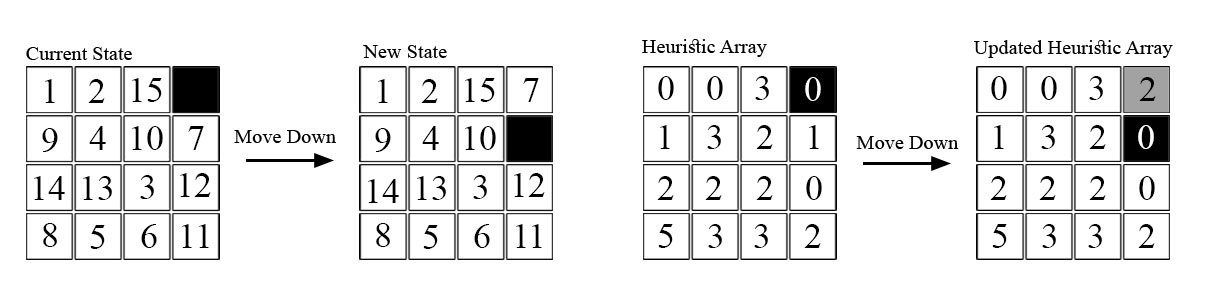
\includegraphics[width=1.1\textwidth]{heuristic_array}
	\captionsetup{justification=centering}
	\caption{A representation of a heuristic array}
	\label{fig:heuristic_array}
\end{figure}



\begin{algorithm}
	\caption{Single Manhattan Distance}\label{Manhattan Distance2}
	\begin{algorithmic}[1]
		\State $heuristicArray$ \Comment{Array where each element has its respected tiles Heuristic value}
		\State $heuristicTotal$ \Comment{The sum of all elements in the heuristic array}
		\State$dimensions$ \Comment{The dimensions of the puzzle e.g 3 for 3x3 and 4 for 4x4}
		\State $movedPosition$ \Comment{The position of the tile that previously swapped with the blank}
		\State $zeroPosition$ \Comment{The current position of the blank tile}
		\Procedure{SingleManDist}{$state$}	\Comment{The current puzzle configuration }
		\State $tileValue\gets state[i]$
		\State $expectedRow\gets (tileValue -1)\div dimensions$
		\State $expectedCol\gets (tileValue -1)\mod dimensions$
		\State $rowNum \gets i\div dimensions$
		\State $colNum\gets i \bmod dimensions$
		\State $tempTotal \gets heuristicTotal \texttt{-} heuristics[zeroPosition]$ 
		\State $newHeuristicValue\gets \mid{expectedRow-rowNum}\mid\texttt{+}\mid{expectedCol-colNum}\mid$
		\State $heuristics[movedPosition]\gets newHeuristicValue$
		\State $heuristics[zeroPosition]\gets 0$
		\State $total \gets tempTotal\texttt{+}newHeuristicValue$
		\State \textbf{return} $total$\Comment{The heuristic estimate of the state is the total}
		\EndProcedure
	\end{algorithmic}
\end{algorithm}



\subsection{Linear-Conflict}
The Linear-Conflict heuristic was implemented by table lookup with one entry for each permutation of a row or column, storing the corresponding linear conflict. Even for the 15-puzzle, there are only 24 permutations of 4 tiles in a row or column. So the cost of the linear-conflict implementation is only a small number of table-lookups. \cite{hansson1992criticizing} implementation showed that on average each calculation of the linear-conflict caused the search program for the fifteen puzzle to be only 5\% slower in examining each node, and this was more than compensated for their dramatic decrease in the number of nodes that needed to be examined when using the linear-conflict heuristic.


\subsection{A*}
A* begins by declaring two empty sets: $closedSet$ stores states that have already been visited; $openSet$ contains states to be visited. The initial state is added to the $openSet$, similar to BFS the $openSet$ is iterated through until it finds a goal state or there are no more states to explore, implying no solutions. The most promising state is retrieved from the $openSet$ (the state with the lowest $F$ score) and assigned to $currentState$. This state is then removed from the $openSet$ and added to the $closedSet$. The $currentState$ is checked to see whether it matches the goal state and returned if so. From the $currentState$ all the possible moves are found and denoted as $neighbours$, each $neighbour$ is checked against the $closedSet$ to make sure the state hasn't already been expanded. The $neighbour$ is then checked against the $openSet$ and if the $openSet$ contains $neighbour$ the $G$ values are compared to check which version of the state has the best route from the starting position see Algorithm~\ref{Astar}.

\begin{algorithm}
	\caption{A*}\label{Astar}
	\begin{algorithmic}[1]
		\State $g(state)$ \Comment The cost to reach the current state
		\State $h(state)$ \Comment Estimated cost of the cheapest path from state to goal
		\State $f(state) \gets g(state)+h(state)$
		\State $neighbours(state)$ \Comment Expands possible moves from current state ordered by g + h
		
		\Procedure{AStar}{$startState$}
		\State $closedSet \gets \textit{empty set}$
		\State $openSet \gets \textit{empty set}$
		\State $openSet.add(startState)$
		\While{$openSet \textbf{ is not } empty$}
		\State $currentState \gets state\   \textbf{in}\ openSet\ with\ lowest\ f\ value$
		\State $openSet.remove(currentState)$
		\State $closedSet.add(currentState)$
		\If {$currentState = goal$}
		\State \textbf{return} $currentState$
		\EndIf
		\For{$neighbour \textbf{ in } neighbours(currentState)$}	
		\If{$neighbour \textbf{ not in } closedSet$}
		\If{$neighbour \textbf{ in } openSet$}
		\If{$g(currentState) < g(neighbour)$} 
		\State$g(neighbour) \gets g(currentState)$
		\EndIf	
		\Else
		\State $openSet.add(neighbour)$	
		\EndIf
		\EndIf
		
		\EndFor
		\EndWhile
		\EndProcedure
	\end{algorithmic}
\end{algorithm}


\subsection{IDA*}

The IDAStar algorithm is very similar to to DFID; IDAStar iteratively deepens dependent on the $F$ value rather than a fixed depth. The initial $bound$ is assigned to the $F$ score of state, which is also just the $H$ value as $G$ is inherently 0 as no moves have been made to get to this state. A depth-first limited search is then executed to the specified threshold. If the $F$ value of the current state is greater than the $bound$ this is returned and assigned to the new $bound$. If the $H$ estimate of the state is 0, no more moves are required to get to the goal state thus the solution is found. Similar to A* the neighbour with the smallest $F$ value is prioritised see Algorithm \ref{IDAStar}.	
\begin{algorithm}
	\caption{Iterative Deepening A Star}\label{IDAStar}
	\begin{algorithmic}[1]
		
		\State $state$ \Comment The current puzzle configuration
		\State $g(state)$ \Comment The cost to reach the current state
		\State $h(state)$ \Comment Estimated cost of the cheapest path from state to goal
		\State $f(state) \gets g(state)+h(state)$
		\State $neighbours(state)$ \Comment Expands possible moves from current state ordered by g + h
		\Statex
		\Procedure{IDAStar}{$state$}
		\State $bound \gets f(state)$
		\While{ \textbf{ not } found}\Comment{Loops until a solution is found}
		\State $ bound \gets DLS(state, bound)$	\Comment Performs a bounded depth-first search 
		\EndWhile\label{}
		\EndProcedure
		\Statex
		
		\Procedure{DLS}{$state, bound$}
		\If{$f(state) > bound$}
		\State \textbf{return} $f(state)$
		\EndIf	
		
		\If{$h(state) = 0$} \Comment No more moves needed to reach goal state
		\State \textbf{return} $found$
		\EndIf
		\State $min \gets \infty$	
		\For{$neighbour \textbf{ in } neighbours(state)$}	
		\State $temp \gets DLS(neighbour, bound)$
		
		\If{$temp < min}$
		\State $min \gets temp $
		\EndIf
		\EndFor
		\State \textbf{return} $min$\Comment{Returns the smallest of the neighbours}
		\EndProcedure
		
	\end{algorithmic}
\end{algorithm}

\subsection{Design of Java Application}
The Java application will run by initially providing the user with two possible inputs: initial/starting state and goal state (optional). The user will then be able to choose which algorithm they would like to use to solve the problem and which heuristic (provided an informed algorithm). Upon completion, the path from the initial state to the goal state will be displayed along with various statistics: time taken, nodes expanded, no. moves and memory used. Initial preprocessing will be done to ensure that the states provided are actually solvable by checking the parity and the length of each state. The program is generic, so can be used to solve any puzzle provided the initial state, goal state and legal moves have been issued.

\subsubsection{Swing}
Swing is a set of program components for Java that enable the possibility of creating graphical user interfaces (GUI) components. Swing was used to allow for a more user-friendly program and display a frame for the results to placed. Also a visual representation of how the program solved the puzzle state will be displayed.
\begin{figure}[h!]
	\centering
	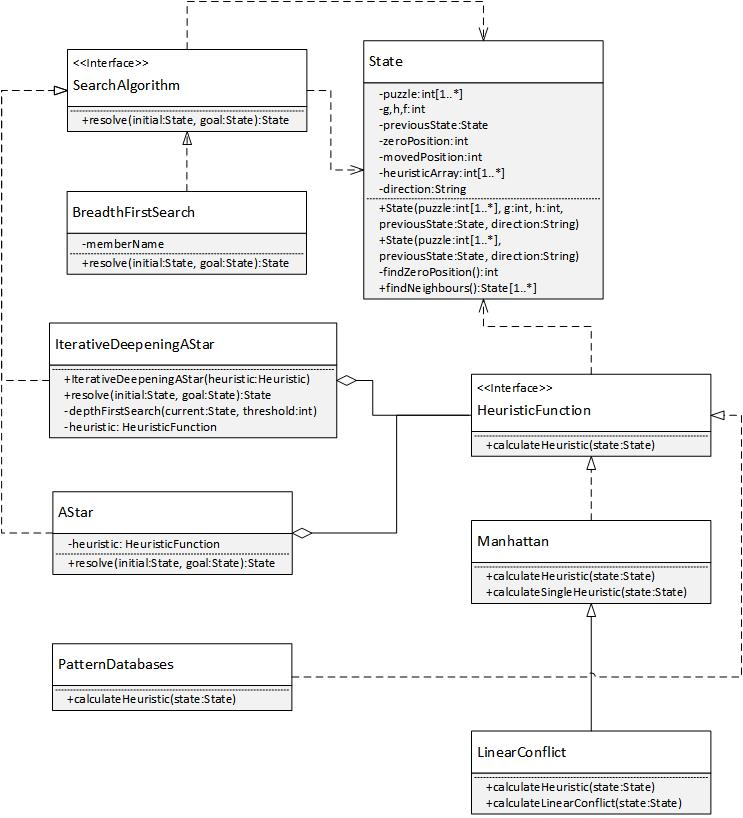
\includegraphics[width=1.1\textwidth]{classDiagram}
	\captionsetup{justification=centering}
	\caption{Class Diagram}
\end{figure}
\section{Implementation}
This section covers the main aspects of the implementation of the project, icluding details on how the algorithms were implemented, as well as the methods used and the implementation details of these methods.





\subsection{Structure}

When a node is being expanded it is necessary to find its neighbours. Neighbours for the sliding-tile puzzle represent the possible moves from the current configuration, each state has a minimum of 2 neighbours and a maximum of 4. Figure 1 shows the possible moves from current state and how the direction variable would be stored ready for output; movements are relative to the blank meaning the variable is represented by the direction the blank moves. The \textit{findNeighbours()} method returns a list of the current state's child nodes. 

The strategy or policy pattern is a behavioural design pattern that enables behaviour to be selected at runtime. The strategy pattern was used in the implementation as shown by Figure \ref{figure:classDiagram}. The family of algorithms was defined by using the \textit{SearchAlgorithm} interface, which defines the \textit{resolve(initialState:State, goalState:State)} which is then further implemented by the specific search classes. Strategy ensures encapsulation of each algorithm and makes the family of algorithms interchangeable \cite{gamma1995design}. Similar to \textit{SearchAlgorithm}, \textit{HeuristicFunction} encapsulates the heuristic functions \textit{Manhattan}, \textit{LinearConflict} and \textit{PatternDatabases}. The \textit{LinearConflict} class is a child to \textit{Manhattan} and performs a super method call to retrieve the Manhattan heuristic estimate for the state, then adds the linear-conflict on top.

\begin{figure}[ht]
	\centering
	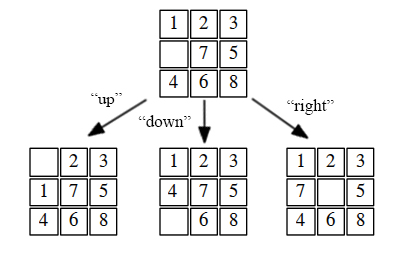
\includegraphics[width=0.5\textwidth]{moves}
	\captionsetup{justification=centering}
	\caption{Finding possible moves}
	\label{figure:classDiagram}
\end{figure}


\subsection{Experimental Plan}
The experiments in this paper vary dependent on the size of the problem domain; a complete experiment was performed on the 8-puzzle, testing each and every possible state in terms of time, expanded nodes, and number of moves taken to reach the goal state.
\subsubsection{Preliminaries}
In order to generate testing states it is important to ensure that the state is solvable. Problem domains may have constraints that can preclude parts of the search space. For example, although the eight puzzle has $9!$ possible positions, only one half of them can be reached from the goal. \citep{DBLP:journals/ci/CulbersonS98}. To determine whether a sliding-tile puzzle is solvable we must calculate the sum of the inversions.
An inversion is when a tile precedes another tile with a smaller number. 
Algorithm~\ref{Solvable} was used to create testing states for the sliding-tile puzzle, states with randomised permutations were constructed and then checked to see if they were solvable, once a total of 10000 solvable test cases were created the search algorithms were then experimented with.
\begin{algorithm}
	\caption{Is Current State Solvable}\label{Solvable}
	\begin{algorithmic}[H]
		\Procedure{IsSolvable}{state}
		\State $puzzleLength \gets state.size()$
		\State 	$gridWidth \gets \sqrt{puzzleLength}$
		\State $blankRowEven \gets true$
		\For{$i\gets 1, puzzleLength$}
		\If{$state[i] =0$}
		\State $blankRowEven \gets (i / gridWidth) \bmod 2 = 0$
		\State $\textbf{continue} $
		\For{$j\gets i + 1, puzzleLength$}
		\If{$state[i] > state[j] \textbf{ and } state[j] \not= 0 $}
		\State $parity \gets !parity$
		\EndIf
		\EndFor
		\EndIf 
		\EndFor
		
		\If{$gridWidth \bmod 2 = 0 \textbf{ and } blankRowEven$}
		\State \textbf{return} $!parity$
		\EndIf
		\State \textbf{return} $parity$
		
		\EndProcedure
	\end{algorithmic}	
\end{algorithm}	


\section{Experimental Results}\label{Experimental Results}
To further explore the algorithms discussed a series of experiments were executed to analyse their performance to make an empirical comparison. 




\subsection{8-Puzzle}
The initial puzzle tested was the 8-puzzle as its small number of solvable states allows for the use of unintelligent search and gives rise to the opportunity of comparison to intelligent search; the 15-puzzle has too large a search space to make a credible comparison. 






\subsubsection{BFS}

Figure \ref{figure:figss} displays the distribution of states in the 8-puzzle: the minimum number of moves to solve the state and the number of existing alternate states which require the same amount of moves. It also displays the results of the summed time taken to solve all of these particular states using BFS.  

Table \ref{table:kysymys} displays the results of the 8-puzzle using breadth-first search. The tests were performed on all $9!/2=181440$ states, an initial BFS was executed from the goal configuration and each state along with the number of moves required was stored. States were split up into testing lists dependent on the number of moves as shown by column 1 and 2. Tests were then executed using breadth-first search on each state, column 3 displays the average number of nodes expanded before finding the goal state, column 4 is the average time taken to solve a given state and column 5 shows the total time taken to solve all states in the specific testing list.
\begin{table}[ht]
	\caption{Breadth-First Search Analysis: 8-puzzle (10000 Random States)}
	\label{table:bfsRandom}
	\begin{center}
		\begin{tabular}{crr} \hline
			Average Moves & Avg Nodes Expanded & Avg. Time(ms)\\ \hline
			21.7142$\pm$0.065 & 89201.4297 & 29.7373\\ \hline
		\end{tabular}
	\end{center}
\end{table}
\begin{figure}[!ht]
	\begin{subfigure}[t]{0.5\textwidth}
		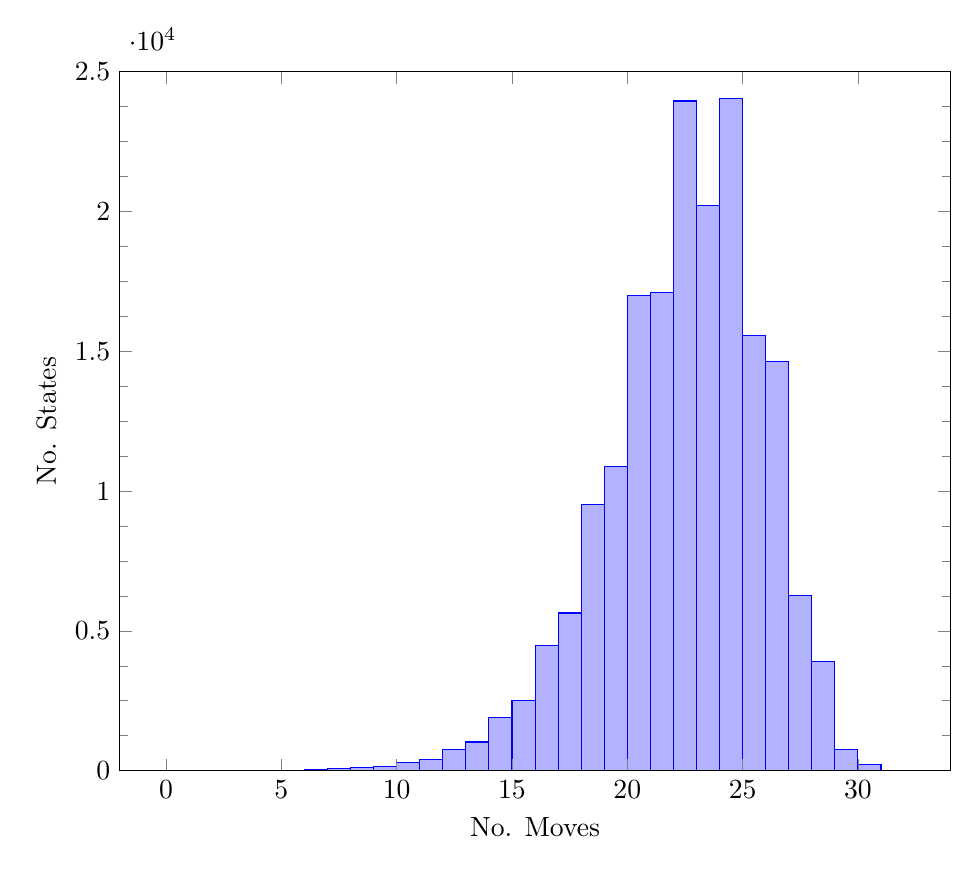
\begin{tikzpicture}
		\begin{axis}[
		width=\textwidth,
		ymin=0, ymax=25000,
		minor y tick num = 3,
		area style,
		xlabel = No. Moves,
		ylabel = No. States,
		]
		\addplot+[ybar interval,mark=no] plot coordinates { 	
			(1,2)
			(2,4)
			(3,8)
			(4,16)
			(5,20)
			(6,39)	
			(7,62)
			(8,116)
			(9,152)
			(10,286)
			(11,396)
			(12,748)
			(13,1024)
			(14,1893)
			(15,2512)
			(16,4485)
			(17,5639)
			(18,9529)
			(19,10878)
			(20,16993)
			(21,17110)
			(22,23952)
			(23,20224)
			(24,24047)
			(25,15578)
			(26,14650)
			(27,6274)
			(28,3910)
			(29,760)
			(30,221)
			(31,2)		 };
		\end{axis}
		\end{tikzpicture}
	\end{subfigure}
	\begin{subfigure}[t]{0.5\textwidth}
		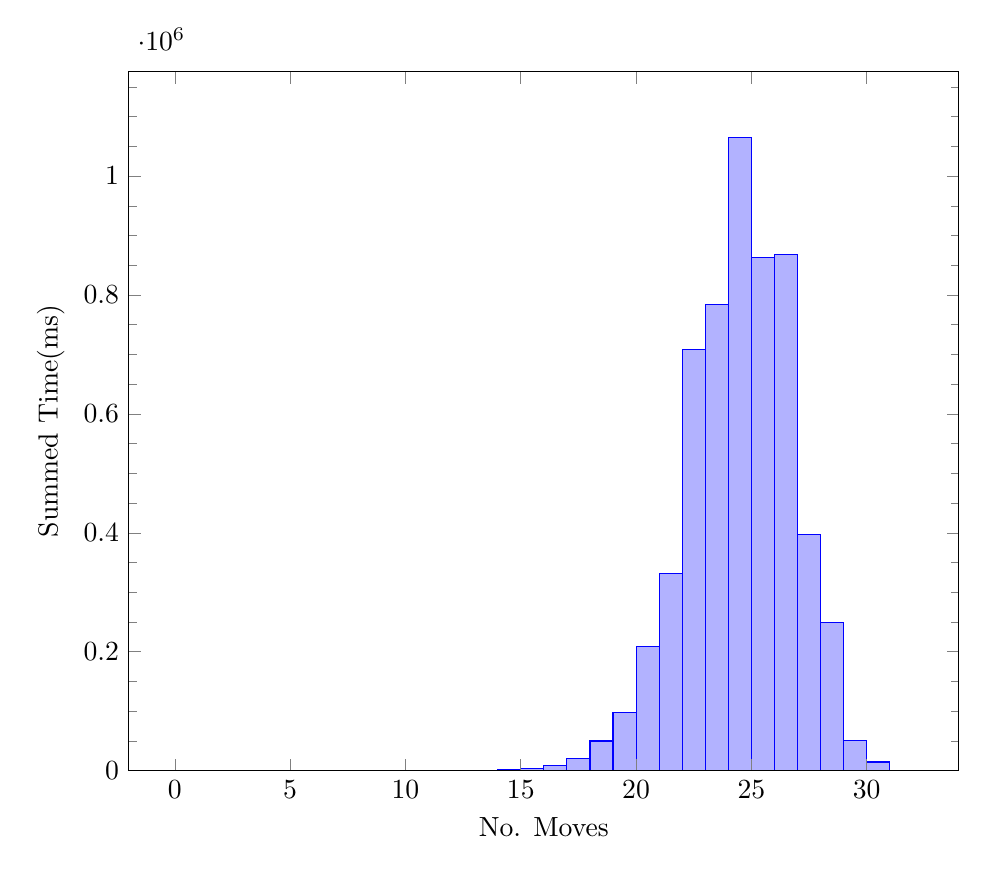
\begin{tikzpicture}
		\begin{axis}[
		width=\textwidth,
		ymin=0, ymax=1175494,
		minor y tick num = 3,
		area style,
		xlabel = No. Moves,
		ylabel = Summed Time(ms),
		]
		\addplot+[ybar interval,mark=no] plot coordinates{
			(1,0)
			(2,0)
			(3,0)
			(4,0)
			(5,2)
			(6,3)	
			(7,8)
			(8,19)
			(9,30)
			(10,61)
			(11,108)
			(12,251)
			(13,587)
			(14,1554)
			(15,3358)
			(16,9354)
			(17,19800)
			(18,49859)
			(19,98138)
			(20,209503)
			(21,330907)
			(22,708861)
			(23,784197)
			(24,1065494)
			(25,862847)
			(26,867818)
			(27,396454)
			(28,248861)
			(29,50164)
			(30,14541)
			(31,133)
		};
		\end{axis}
		\end{tikzpicture}
	\end{subfigure}%

	\caption{A representation of the number of states that require a specific amount of moves to be solved optimally in the 8-tile and the summed time taken for all these states to be solved}
	\label{figure:figss}
\end{figure}
\begin{table}[ht]
	\caption{Breadth-First Search Analysis: 8-puzzle}
	\label{table:kysymys}
	\begin{center}
		\begin{tabular}{crrrr} \hline
			Min Moves & No. States & Avg Nodes Expanded & Avg. Time(ms) & Total Time(ms) \\ \hline
			0-4  & 31 & 747.19$\pm$435.76 & 0.5483 & 18 \\
			5-9 & 389 &4249.35$\pm$4277.99& 1.0668 & 432.0 \\ 
			10-14 & 4347 &  23257.75$\pm$20745.99& 5.7888 & 25164  \\ 
			15-19 & 33042& 58446.06$\pm$35484.49 & 17.7823 & 587563 \\ 
			20-24 & 102326& 114724.84$\pm$36410.64 & 41.0058 & 4195959  \\ 
			25-29 & 41082& 162772.14$\pm$15654.31 & 60.0550 & 2467181 \\ 
			30+ & 223& 180524.70$\pm$548.90 & 67.3542 & 15006\\ \hline
		\end{tabular}
	\end{center}

\end{table}




\begin{figure}[!ht]
	\centering
	\begin{subfigure}[t]{0.5\textwidth}
		\begin{tikzpicture}
		\begin{axis}[
		width=\textwidth,
		xlabel = No. Moves,
		ylabel = Average Time(ms),
		]
		\addplot[error bars/.cd, y dir=both, y explicit, ] coordinates{
			(2,0)
			(3,0)
			(4,0)
			(5,0.0625)
			(6,0.07)	
			(7,0.12903)
			(8,0.16379)
			(9,0.19737)
			(10,0.21329)
			(11,0.27273)
			(12,0.33556)
			(13,0.57324)
			(14,0.82092)
			(15,1.33678)
			(16,2.08562)
			(17,3.51188)
			(18,5.23234)
			(19,9.0217)
			(20,12.32878)
			(21,19.33998)
			(22,29.59507)
			(23,38.77556)
			(24,44.30881)
			(25,55.38882)
			(26,59.60288)
			(27,63.18999)
			(28,63.64731)
			(29,66.00526)
			(30,65.79638)
			(31,66.5)
		};
		\end{axis}
		\end{tikzpicture}
	\end{subfigure}%
	\begin{subfigure}[t]{0.5\textwidth}
		\begin{tikzpicture}
		\begin{axis}[
		width=\textwidth,
		xlabel = No. Moves,
		ylabel = Mean Nodes Expanded,
		]
		\addplot[error bars/.cd, y dir=both, y explicit, ] coordinates{
			(1,3.5)
			(2,8.25)
			(3,15.625)
			(4,25)
			(5,46.9)
			(6,79.87179)	
			(7,142.03226)
			(8,222.75)
			(9,396.56579)
			(10,607.36364)
			(11,1033.95707)
			(12,1580.87032)
			(13,2689.3877)
			(14,4068.70417)
			(15,6816.66521)
			(16,10077.94314)
			(17,16304.61352)
			(18,23252.76262)
			(19,35532.59423)
			(20,47973.72595)
			(21,68096.92613)
			(22,86105.56809)
			(23,111406.96737)
			(24,129960.55254)
			(25,151666.94146)
			(26,163973.55021)
			(27,174731.22792)
			(28,178683.9913)
			(29,180883.49474)
			(30,181336.30769)
			(31,181439.5)
		};
		\end{axis}
		\end{tikzpicture}
	\end{subfigure}
	\caption{8-tile analysis using breadth-first search to display how the minimum number of moves required to reach the goal state affects the time(ms) and the number of nodes expanded}
\end{figure} 


\subsubsection{DFID}
Although DFID maintains the advantage of requiring a comparable supply of memory as depth-first search and doesn't get caught in infinite loops, DFID's time taken to find a solution is vast and generally longer than both depth-first search and breadth-first search, this is because it has to expand the same states multiple times. Figure \ref{fig:dfidres} shows the exponential growth of time taken as the number of moves to solve the problem increases.

\begin{figure}[!ht]
	\centering 
	\begin{subfigure}[t]{0.5\textwidth}
		\begin{tikzpicture}
		\begin{axis}[
		width=\textwidth,
		xlabel = No. Moves,
		ylabel = Average Time(ms),
		]
		\addplot[error bars/.cd, y dir=both, y explicit, ] coordinates{
			(2,0)
			(3,0)
			(4,0)
			(5,0)
			(6,0)	
			(7,0)
			(8,0.02586)
			(9,0.07895)
			(10,0.13986)
			(11,0.15404)
			(12,0.2861)
			(13,0.44531)
			(14,0.69625)
			(15,1.13416)
			(16,1.88272)
			(17,3.46577)
			(18,5.53332)
			(19,10.07575)
			(20,16.1287)
			(21,29.60105)
			(22,47.66779)
			(23,89.32199)
			(24,139.81619)
			(25,256.82822)
			(26,405.10041)
			(27,745.5569)
			(28,1133.44041)
			(29,2094.95789)
			(30,3076.80543)
			(31,5706.5)
		};
		\end{axis}
		\end{tikzpicture}
	\end{subfigure}%
	\caption{8-tile analysis using DFID to display how the minimum number of moves required to reach the goal state affects the time(ms) and the number of nodes expanded}
	\label{fig:dfidres}
\end{figure} 


\begin{table}[ht]
	\caption{Depth-First Iterative Deepening: 8-Tile}
	\begin{center}
		\begin{tabular}{crrr} \hline
			Min Moves & Moves & Nodes Expanded &Time(ms)  \\ \hline
			5  & 5 & 56 & 0.9521 \\
			10 & 10  &6392&  16.777216 \\ 
			15 & 15 & 3350884& 2902.4583  \\ \hline
			
		\end{tabular}
	\end{center}
\end{table}



\subsubsection{A*}
A* was the first informed search to be tested using both the Manhattan distance heuristic and the linear conflict. Every possible permutation of the puzzle was tested using the A* with Manhattan distance and A* with Manhattan distance + Linear Conflicts, to compare the results and analyse how much linear conflict tightens the lower bound of the estimate. Figure \ref{Figure:astar} displays the results of A* with an increasing number of moves using Manhattan distance as the heuristic estimator, the graphs show a clear exponential growth on the y axis, both in the same taken to solve the state and the average number of nodes expanded. When the number of moves required to solve the state reached 31 (The maximum number of moves to solve any sliding tile state) there is a decline in the average time taken and the average number of nodes expanded. But as there are only two states in the puzzle which require 31 moves to solve no empirical conclusion can be made until tests are performed on puzzles with a larger domain.


\begin{figure}[!ht]
	\centering
	\begin{subfigure}[t]{0.5\textwidth}
		\begin{tikzpicture}
		\begin{axis}[
		width=\textwidth,
		xlabel = No. Moves,
		ylabel = Average Time(ms),
		]
		\addplot[error bars/.cd, y dir=both, y explicit, ] coordinates{
			(2,0)
			(3,0)
			(4,0)
			(5,0)
			(6,0)	
			(7,0)
			(8,0)
			(9,0.00658)
			(10,0.00699)
			(11,0.01515)
			(12,0.01872)
			(13,0.02246)
			(14,0.03117)
			(15,0.05454)
			(16,0.08361)
			(17,0.13515)
			(18,0.21052)
			(19,0.35999)
			(20,0.56906)
			(21,1.07873)
			(22,1.76144)
			(23,3.55662)
			(24,6.26918)
			(25,13.28245)
			(26,23.95968)
			(27,53.01833)
			(28,93.68286)
			(29,203.16579)
			(30,320.31674)
			(31,232)
		};
		\end{axis}
		\end{tikzpicture}
	\end{subfigure}%
	\begin{subfigure}[t]{0.5\textwidth}
		\begin{tikzpicture}
		\begin{axis}[
		width=\textwidth,
		xlabel = No. Moves,
		ylabel = Mean Nodes Expanded,
		]
		\addplot[error bars/.cd, y dir=both, y explicit, ] coordinates{
			(1,2)
			(2,3)
			(3,4)
			(4,5)
			(5,6.15)
			(6,7.4359)	
			(7,9.04839)
			(8,10.2931)
			(9,12.48684)
			(10,15.34266)
			(11,19.79545)
			(12,25.60963)
			(13,35.62988)
			(14,46.79345)
			(15,67.2711)
			(16,87.57547)
			(17,125.84622)
			(18,163.32039)
			(19,235.00414)
			(20,306.49632)
			(21,441.65073)
			(22,577.32536)
			(23,840.73507)
			(24,1107.93692)
			(25,1616.53916)
			(26,2129.70076)
			(27,3127.82898)
			(28,4065.00639)
			(29,6103.83026)
			(30,7995.22172)
			(31,7282)
		};
		\end{axis}
		\end{tikzpicture}
	\end{subfigure}
	\caption{8-tile analysis using A star search to display how the minimum number of moves required to reach the goal state affects the time(ms) and the number of nodes expanded}
	\label{Figure:astar}
\end{figure} 

\begin{table}[ht]
	\caption{A*: 8-puzzle (10000 Random States)}
	\begin{center}
		\begin{tabular}{crr} \hline
			Average Moves & Avg Nodes Expanded & Avg. Time(ms)\\ \hline
			21.7142$\pm$0.065 & 958.989 & 9.8062\\ \hline
		\end{tabular}
	\end{center}
\end{table}


\subsubsection{Manhattan Distance and Linear Conflict}
Tests displayed in Table 4 show that A* search with the linear conflict heuristic improves the performance of A* with Manhattan distance for the 8-tile puzzle. On average A* with linear conflict would take around 1ms longer than A* with Manhattan distance, until the number of moves required to solve the puzzle were greater than 25, as this showed a substantial decline in time when comparing the linear conflict to the Manhattan heuristic. This implies that the performance of linear conflict exceeds the performance of Manhattan distance when the state space grows, so the more difficult the puzzle the greater the gap in performance between the two heuristics becomes.

As the state space grows exponentially according to the depth the growth is smaller for the A* with linear conflict, this is because the heuristic is a more accurate representation of the displacement of the tiles, thus the H value is always larger than or equal to the H value of the Manhattan Distance. Table 5 shows the difference in H value for 10 calculations of both algorithms and how the linear conflict is nearly always larger than the Manhattan distance.

Table 4 shows the exponential growth by the number of states the algorithm expanded. The average number of States for the Manhattan distance heuristic from 5 to 30 moves is 972.5, whereas linear conflict's average is 651.




\subsection{15-Puzzle}

Initially, the A* Manhattan distance and the A* linear conflict  was implemented for the fifteen tile puzzle, the algorithm struggled due to the number of states required to be stored in the closed set. 

A* uses breadth-first traversal thus the number of states that are stored increases exponentially with depth. Finding an algorithm which would require less memory but still had the benefits of a heuristic search was necessary. This is similar to the previous scenario when considering how to reduce the memory used in breadth-first by taking depth-first search's memory used as inspiration.

The memory used by Depth-first iterative deepening is linear with respect to the depth. In theory DFID could be used to solve the 15-puzzle without running out of memory, however taking the results found in Table 3, the time taken to reach the goal state for any random instance of the fifteen tile puzzle would be unreasonable.


\subsubsection{IDA*}

\captionof{table}{Iterative Deepening A* Results}
\begin{center}
	
	\begin{tabular}{|l|r|r|r|r|} \cline{2-5}
		
		\multicolumn{1}{c}{} & \multicolumn{2}{|c|}{Linear Conflict} &
		\multicolumn{2}{|c|}{Manhattan Distance} \\ \hline
		Min Moves & Time(ms) & States Expanded & Time(ms) & States Expanded \\	\hline \hline
		5  & 2.2913 & 6                        & 2.4060       &          6            \\
		10 & 2.3751  & 13                      & 2.3739       &         11            \\
		15 & 2.8140 & 24                       & 2.5081          &      16            \\
		20 & 11.3692 & 919                     & 8.0932        &        768           \\
		25&  21.9585  & 10420                  & 37.5986        &       25272         \\
		30& 117.3271 & 91471                   & 159.5604        &      217239        \\
		35  & 215.4406 & 231508                & 287.0284        &      482893        \\
		40& 78.972869 & 61141                  & 120.4332          &    110903        \\
		45 & 1750.4441 & 2468006               & 7111.9494        &     14202684      \\
		50& 9162.8202 & 13704525               & 17143.5055         &   36202294       \\
		55 & 6233.2757 & 9132143               & 13912.0609        &    29537720       \\
		60 & 61771.3520 & 87466771             & 277232.1371      &     596363837      \\
		\hline
		
	\end{tabular}
	
\end{center}


\begin{figure}[!ht]
	
	\begin{subfigure}[t]{.5\textwidth}
		\begin{tikzpicture}
		\begin{axis}[
		width=\textwidth,
		axis lines = left,
		xlabel = Min Moves,
		]
		\addplot coordinates{(5,2.5849)(10,3.7)(15,4.5849)(20,9.8439)(25,13.347)(30,16.481)(35,17.8207)(40,15.899)(45,21.234)(50,23.708)(55,23.122)(60,26.382217)};
		
		\addplot
		coordinates{(5,2.5849)(10,3.459)(15,4)(20,9.5849)(25,14.62626)(30,17.72892)(35,18.881)(40,16.7589)(45,23.7596)(50,25.10958)(55,24.81606)(60,29.15162)};
		
		\end{axis}
		\end{tikzpicture}
		\caption{Log Of The States Expanded}
	\end{subfigure}
	\begin{subfigure}[t]{.5\textwidth}
		\begin{tikzpicture}
		\begin{axis}[
		width=\textwidth,
		axis lines = left,
		xlabel = Min Moves,
		]
		\addplot coordinates{(5,1.1961)(10,1.2479)(15,1.492622)(20,3.507059)(25,4.456708)(30,6.874392)(35,7.7511)(40,6.303)(45,10.773)(50,13.161)(55,12.60577)(60,15.91465)};
		
		\addplot
		coordinates{(5,1.2666)(10,1.2472)(15,1.3265)(20,3.01)(25,5.232)(30,7.31795)(35,8.16505)(40,6.912089)(45,12.79603)(50,14.0653)(55,13.76405)(60,18.08073)};
		\end{axis}
		\end{tikzpicture}
		\caption{Log Of The Time}
	\end{subfigure}
	\caption{Logarithmic Comparison Of IDA* Fifteen Tile}
\end{figure}



\subsection{Statically-Partioned Additive Database Heuristics}
The 6-6-3 partitioning  was initially implemented many papers state that it is the best compromise between speed and memory to other possible solutions, Figure \ref{fig:partitioning} displays the used partitioning. The first two images display the fifteen tile with the subsets comprising of 6 tiles, $2\times(16!/(16-6)!)= 11531520$ states to be stored, the final subset requires $16!/(16-3)!=3360$ states stored that's a total of $11534880$ states to that were stored. To get these disjoint groups a BFS was used once and the states was serialised into 3 separate files. When testing, a table lookup was performed and the states were stored into the data structure for testing.

\subsection{Tower of Hanoi}

\section{Conclusion and Evaluation}
\clearpage
\bibliography{bibfile}


\appendix
\clearpage





\end{document}

